% !TEX program = xelatex
\documentclass[a4paper,11pt]{article}
\usepackage{graphicx} % Required for inserting images
\usepackage[]{geometry} % Insert size in the [] to define and control the margins on the page
\usepackage{hyperref} % Makes links and table of contents clickable
\hypersetup{colorlinks=true, linkcolor=blue, urlcolor=blue} 
% Use this if you want the links to be noticeable and have color blue, the color can be changed
% \usepackage{mathtools} % math tools builds upon amsmath, so only one of them is needed, note that mathtools has all the functions that amsmath has and even more
\usepackage{amsmath ,amssymb,amsthm}
\usepackage{tikz}
\usepackage{tikz-cd}
\usepackage{subcaption}
\renewcommand{\qed}{\hfill\blacksquare}
\newcommand{\D}[1]{\Delta #1}
\renewcommand{\a}{\alpha}

% \newcommand{\a}{\alpha}
\usepackage{cancel}
\usepackage{float}
\usepackage{enumitem}
\usepackage[T1]{fontenc}
\usepackage{lmodern}
\usepackage{todonotes}
% \renewcommand{\labelitemi}{$\bullet$} # this also works
\setlist[itemize]{label=$\bullet$}
\newcommand{\ML}[1]{\todo[color=yellow!20,author=\textbf{מתן},inline]{\small #1\\}}
\newcommand{\YS}[1]{\todo[color=blue!20,author=\textbf{יובל},inline]{\small #1\\}}



% ============================================================ %

% HEBREW support via polyglossia %

% ============================================================ %

\usepackage{polyglossia}

\defaultfontfeatures{Mapping=tex-text, Scale=MatchLowercase}

\setdefaultlanguage{hebrew}

\setotherlanguage{english}

\newfontfamily\hebrewfont[Script=Hebrew]{David CLM}

% Use \begin{hebrew} block of text \end{hebrew} for paragraphs.

% Use \texthebrew{ } and \textenglish{ } for short texts.

% ============================================================ %
\newcommand{\te}[1]{\textenglish{#1}}
\usepackage{bidi} % we use bidi for Right-To-Left (RTL) writing
\title{\te{Chronos: Learning the Language of Time Series}}
\author{מתן לבינטוב \and יובל שוורץ \and גבריאל מגידוב \and שי קרנצברג}
\date{}
% Begin of Document ---------------------------------------- %
\begin{document}
\begin{RTL}
    
% Title ---------------------------------------- %
\maketitle
% \newpage
% Table of Contents ---------------------------------------- %
% \tableofcontents
% \newpage
% Start of paper ---------------------------------------- %
\section{תיאור כללי של הרעיון}
אנו לוקחים מודל מאומן מראש של \te{Amazon} שהוא ממשפחת \te{pretrained time series forecasting models} בשם \te{Chronos}. \te{Chronos} הוא מודל חיזוי של סדרות עתיות (\te{Time Series}) שמבוסס על ארכיטקטורה של \te{LLM}. המודל לוקח סדרה עיתית, עושה עליה טרנפורמציות של נתונים כדי להפוך אותה ל \te{context tokens} שאותם הוא שולח למודל השפה שספציפית אומן על סדרות עיתיות. לאחר שמודל השפה קיבל את ה\te{context}, אנו מבקשים ממנו לחזות את ה \te{token} הבא שאותו המודל מחזיר לפורמט המקורי של הסדרה העיתית.
\begin{figure}[H]
    \centering
    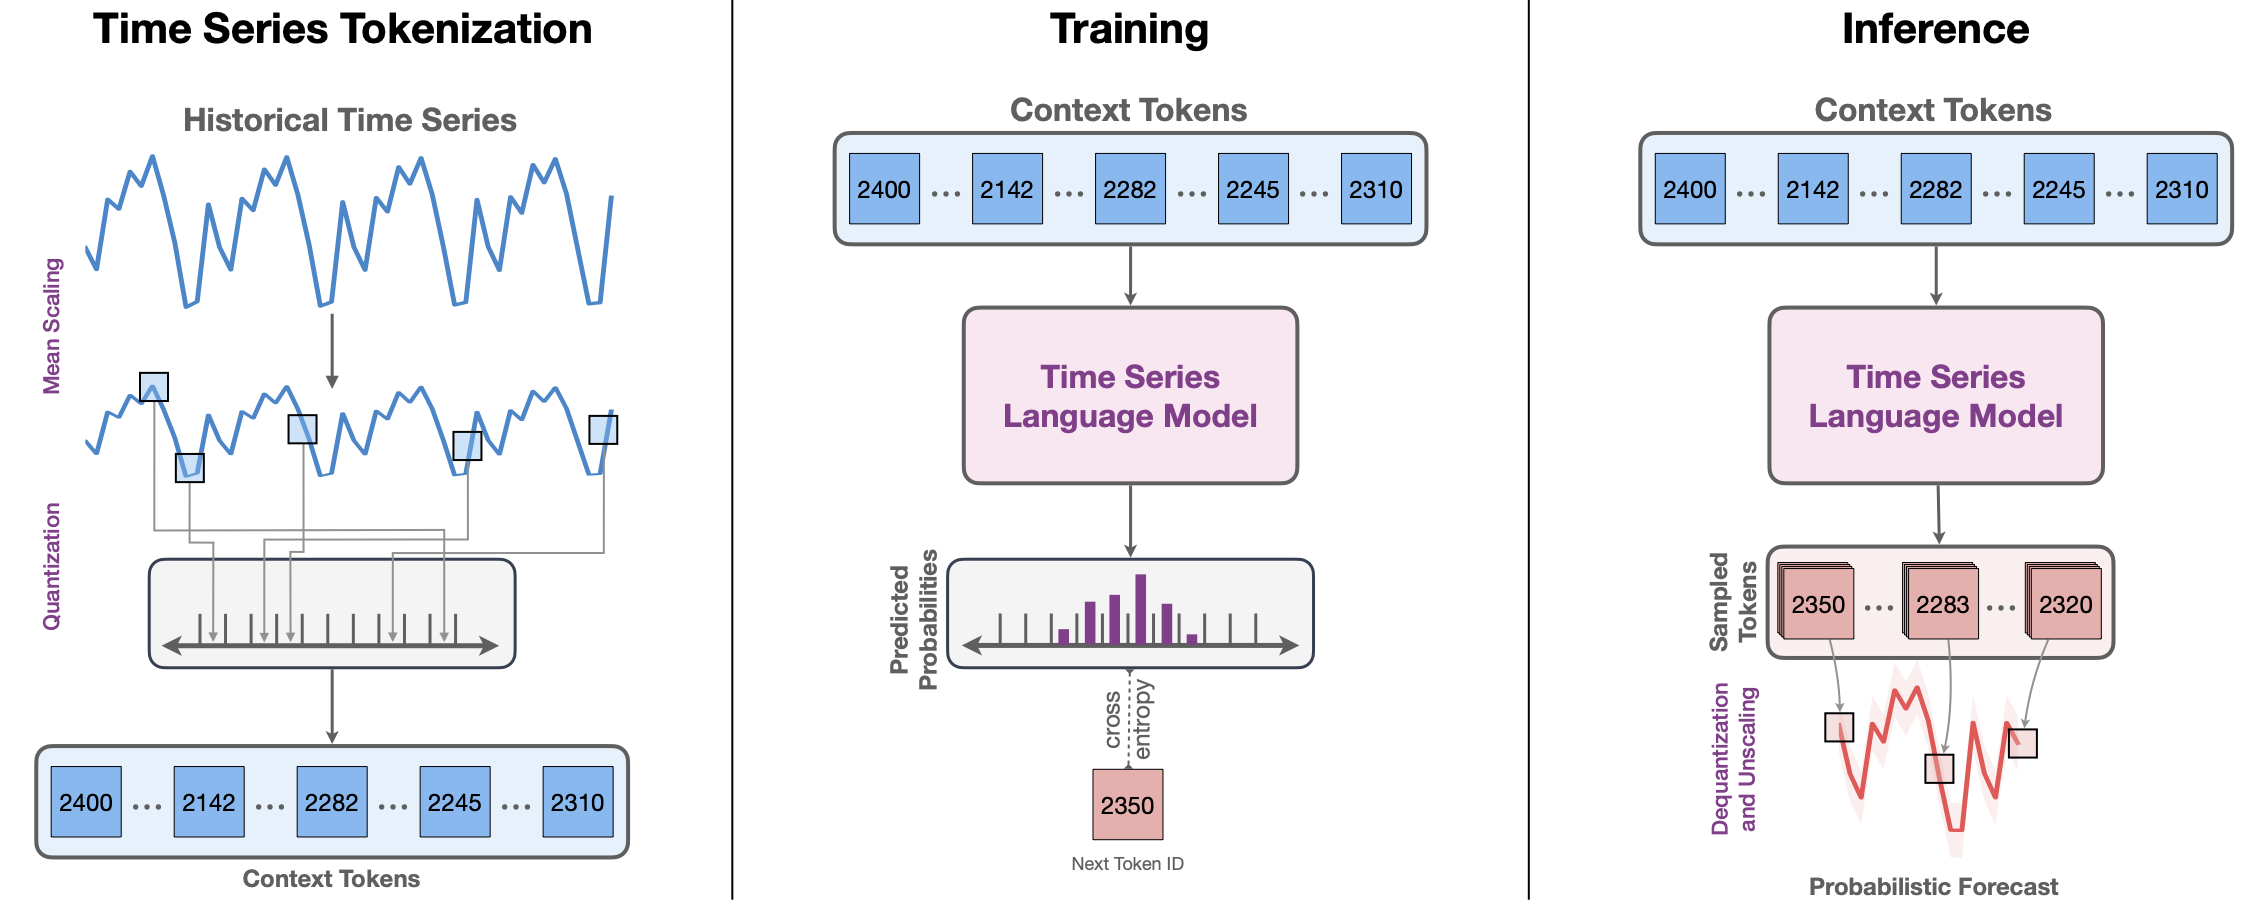
\includegraphics[width=1\textwidth]{Chronos Pretrained Model.png}
    \caption{הארכיטקטורה של \te{Chronos}}
\end{figure}
באמצעות \te{Chronos} ונתוני עבר של \te{Bitcoin} ו \te{Ethereum} אנו מנסים לחזות את מחירי הסגירה של \te{Bitcoin} בנר הבא. מצאנו שהמודל חוזה בצורה אמינה יותר ככל שאנו מביאים לו יותר נתוני עבר רלוונטים וכדי להשתמש ביתרון של \te{Bitcoin}, הנסחר 24/7 וממנו ניתן להשיג נתונים תוך יומיים מפורטים ולכן בחרנו לעבוד עם נרות שעתיים.
\\
בבדיקות שערכנו, מצאנו שיש קורלציה חזקה בין מחירי \te{Bitcoin} למחירי \te{Ethereum}, ולכן החלטנו לנסות להשתמש בשני הנתונים יחדיו ומצאנו שאמינות המודל גדלה.
\\
בנוסף, בחרנו להשתמש באינדיקטור טכני \textenglish{STC - Schaff Trend Cycle Indicator} על מנת לסנן את התחזיות של המודל. \te{STC} הוא אינדיקטור טכני המשלב בין ממוצעים נעים למחזורי זמן כדי לזהות מגמות בשוק בצורה מהירה ומדויקת.
\newpage
\section{פירוט מקורות נתונים}
את הנתונים לקחנו מ \te{Binance}. השתמשנו ב \te{API} שלהם ובספריית \te{requests}, ניתן למצוא את הקוד ב \te{main.py} תחת הפונקציה \te{get\_binance\_historical\_data($\cdot$)}. את הבסיס לפונקציה לקחנו מהמעבדה עם יונתן והתאמנו אותה לצריכנו על ידי הוספת האופציה לתאריך סיום. לקחנו נתוני עבר שעתיים של \te{Bitcoin} ו \te{Ethereum} מסוג \te{OHLCV}.
\begin{figure}[H]
    \centering
    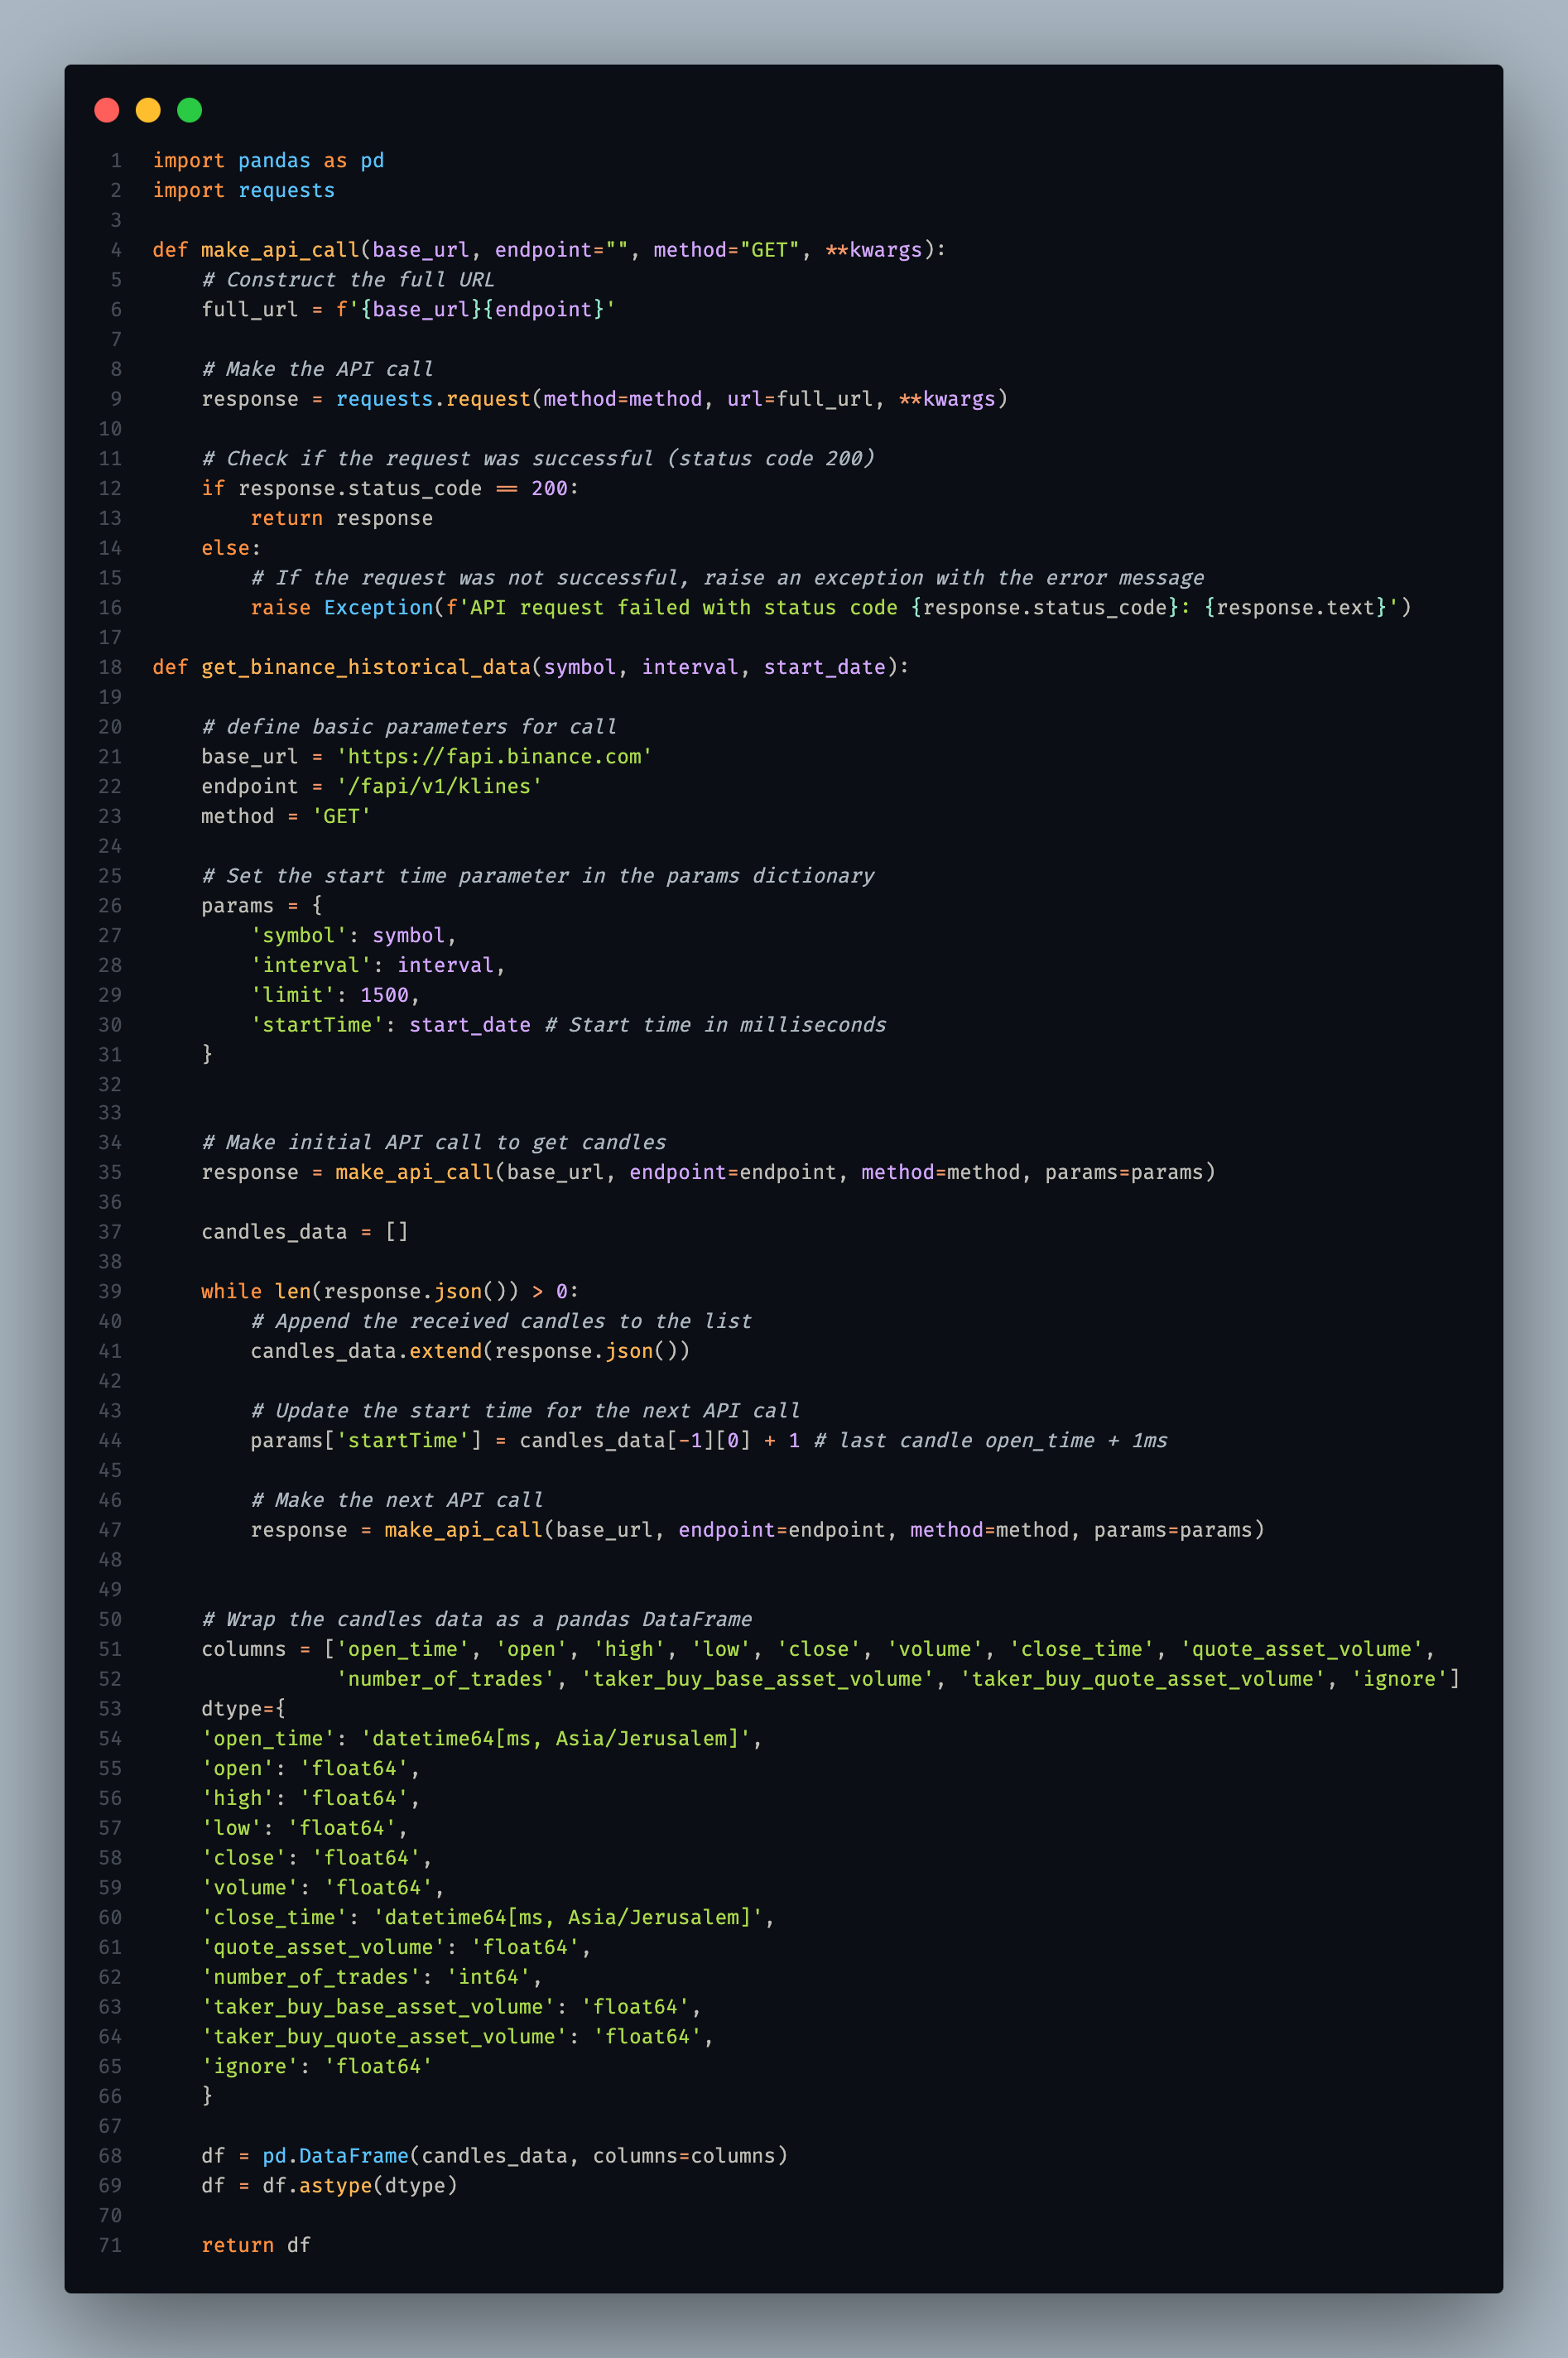
\includegraphics[width=.75\textwidth]{Data.png}
    % \caption{דוגמא לנתוני \te{Bitcoin}}
\end{figure}
\newpage
\section{סטטיסטיקה תאורית של הנתונים והסבר על תהליכי ניקיון וטיוב של הנתונים}
\subsection{סטטיסטיקה תאורית}
\begin{figure}[H]
    \centering
    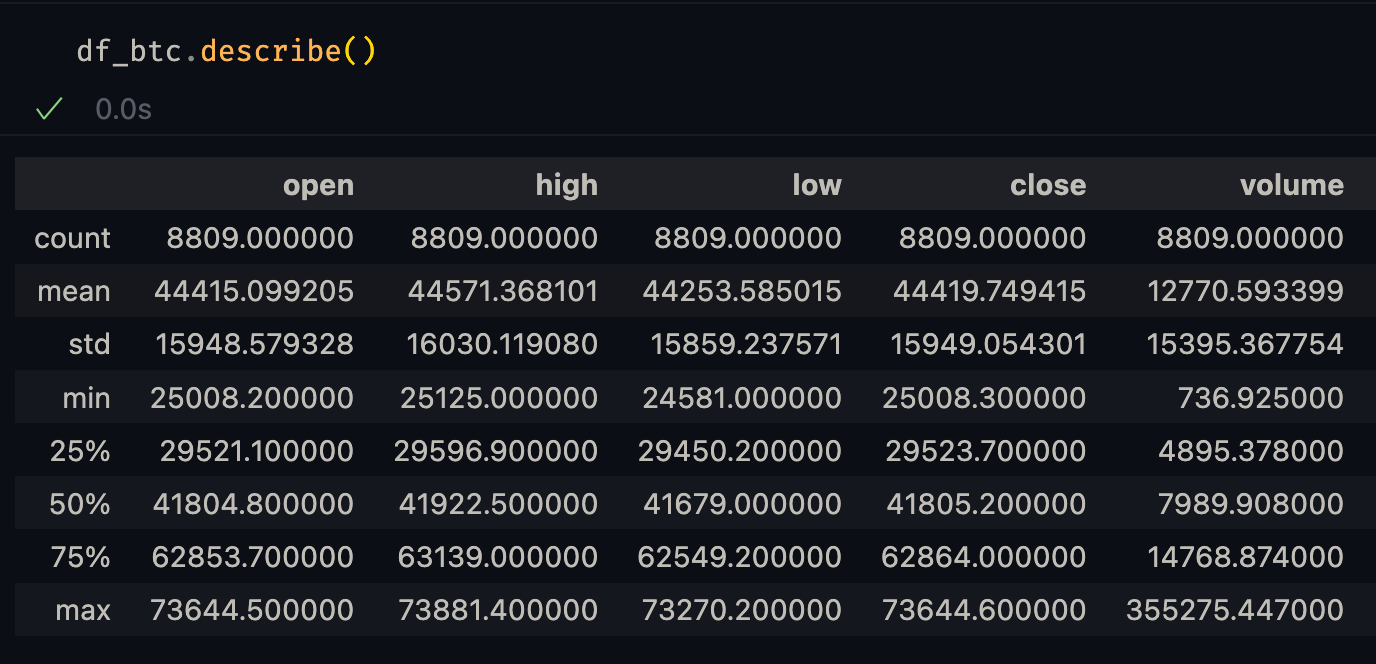
\includegraphics[width=1\textwidth]{bitcoin_stats.png}
    \caption{סטטיסטיקה תאורית של \te{Bitcoin}}
\end{figure}

\begin{figure}[H]
    \centering
    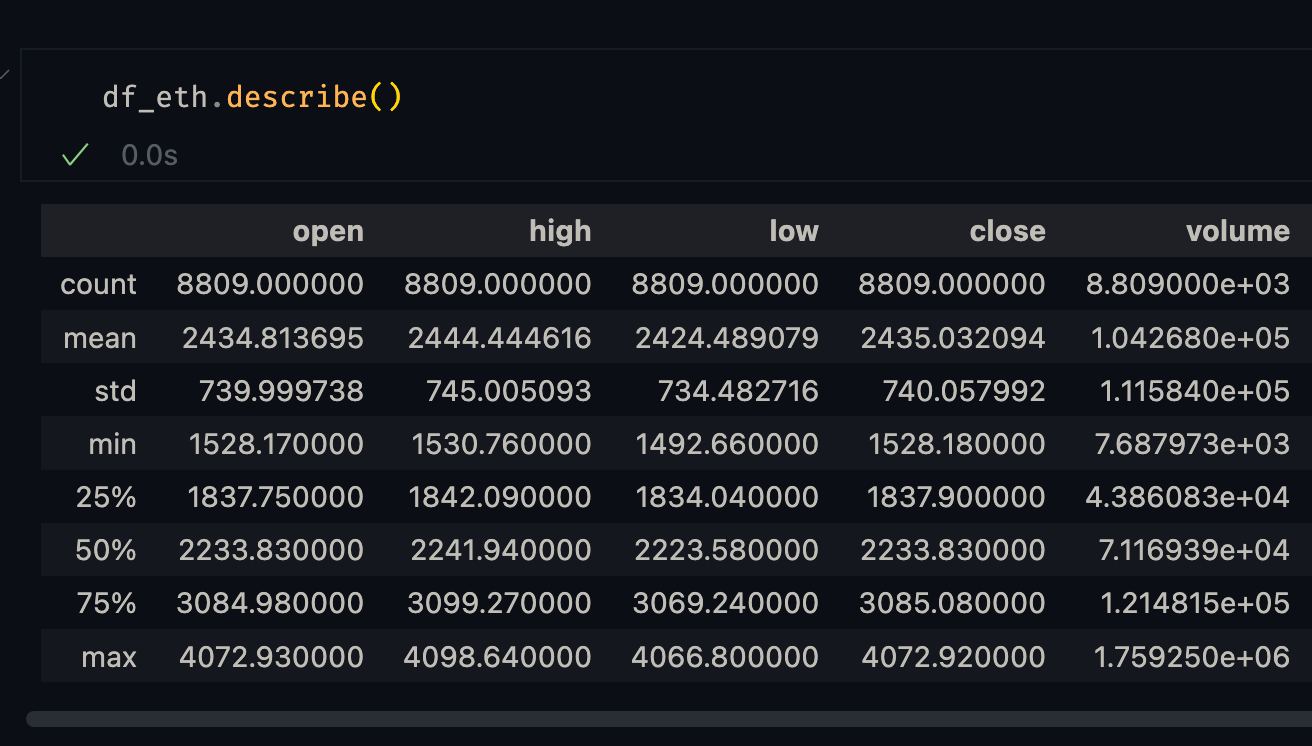
\includegraphics[width=1\textwidth]{ethereum_stats.png}
\caption{סטטיסטיקה תאורית של \te{Ethereum}}
\end{figure}
\subsection{תהליך הניקוי והתיקון}
בקובץ \te{config.json} ניתן לבחור אם המשתמש מעוניין לבדוק ולנקות את הדאטא, כמובן שזה מומלץ ואף חיוני. פונקציית תיקון וניקוי הדאטא עוברת על הדאטא ומחפשת ערכי \te{open / close} שנמצאים מחוץ לטווח \te{low / high} שלהם. כשהיא מוצאת כאלו היא מוחקת את הערך (היא שמה \te{NaN} במקום אותו ערך). לאחר מכן קוראים לפונקציה,\\ \te{mean\_imputation\_without\_leakage($\cdot$)} שהיא מחליפה את הערכים החסרים בממוצע הערכים הקודמים אשר עומדים בטווח (בטווח הכוונה לטווח \te{low / high}).

% \missingfigure{חסר}
\begin{figure}[H]
    \centering
    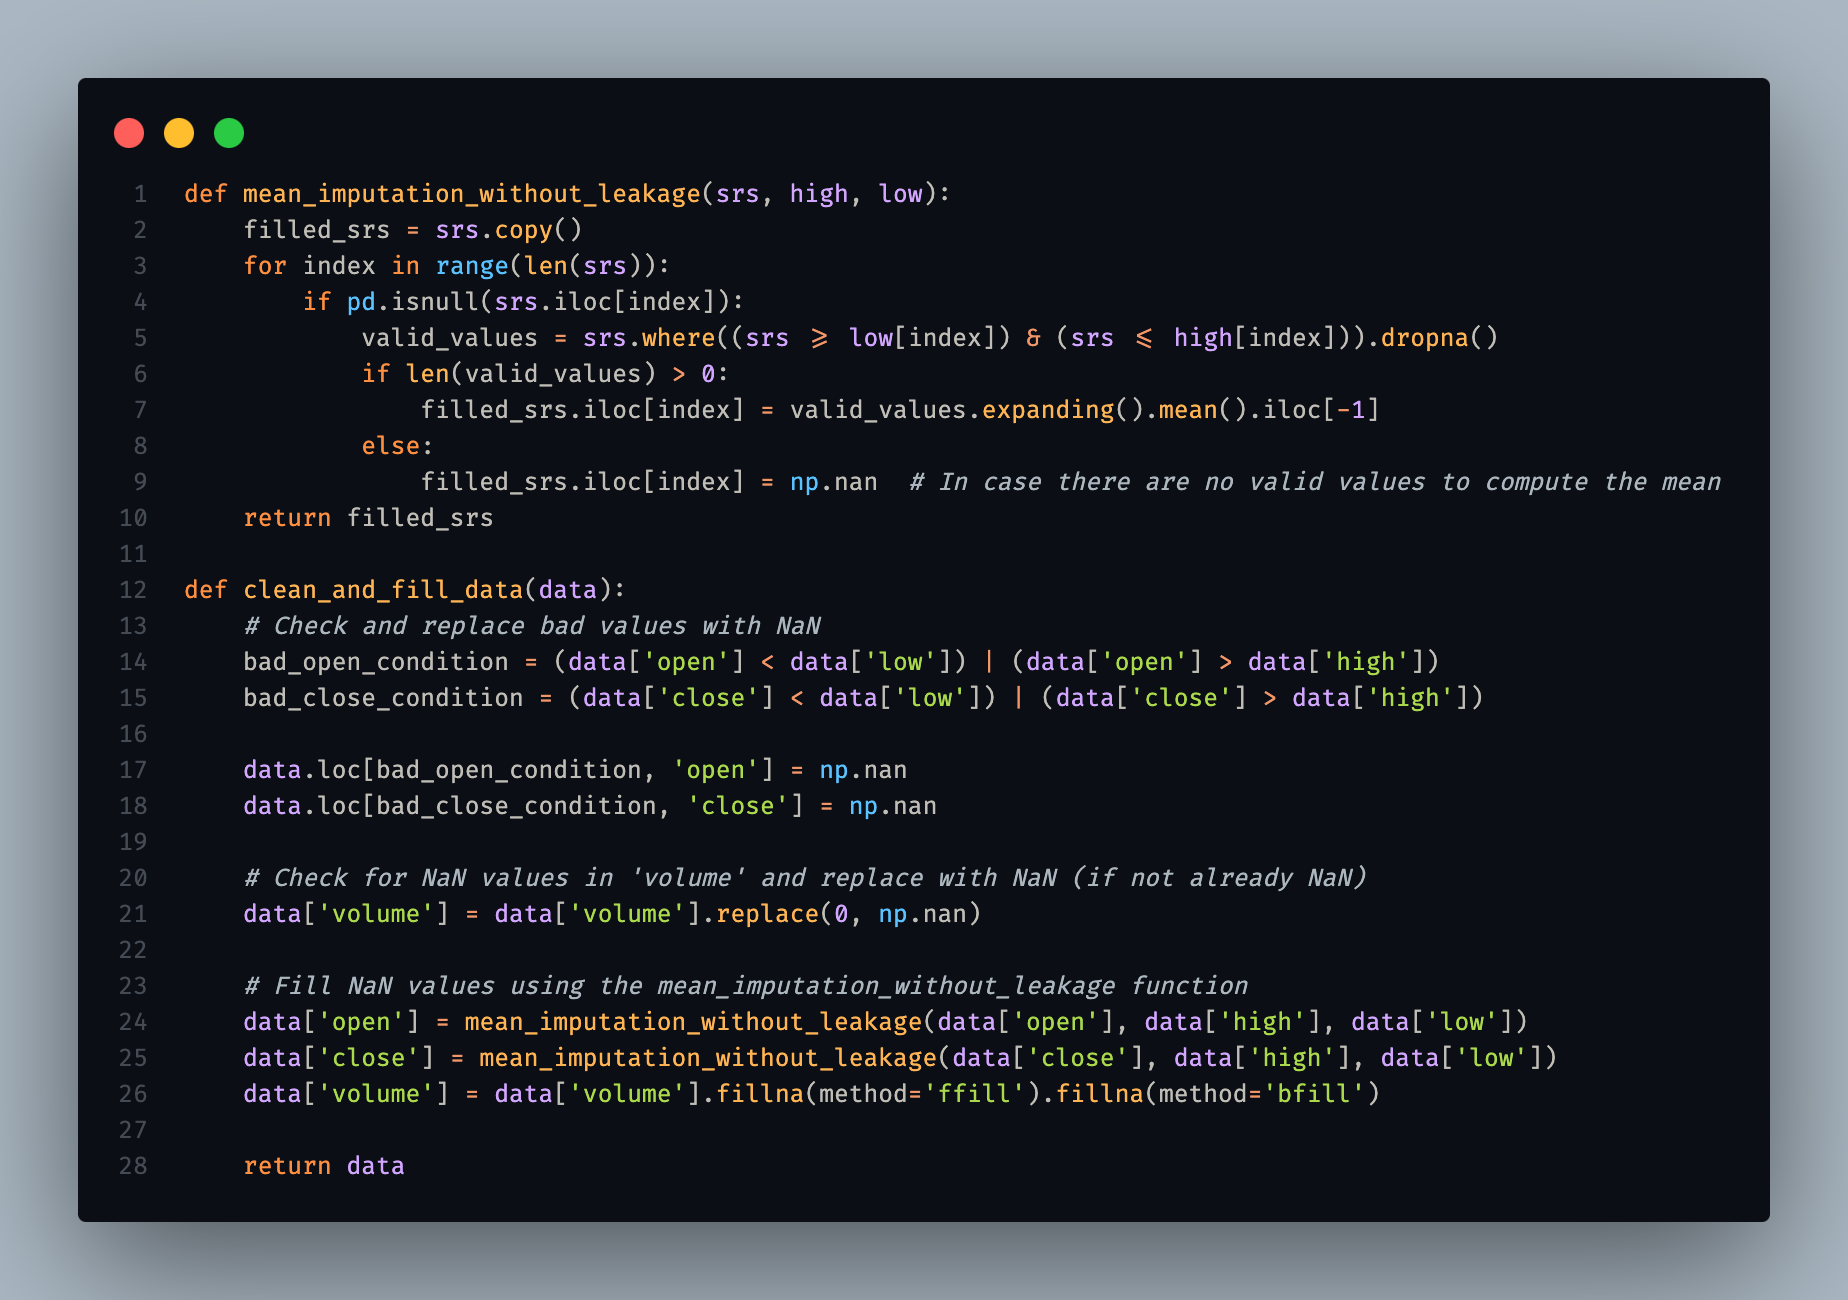
\includegraphics[width=.8\textwidth]{Data_cleaning.png}
    \caption{תהליך ניקוי ותיקון הנתונים}
\end{figure}

\section{תיאור מפורט של האסטרטגיה}


בכל נקודת זמן, אנחנו שולחים \te{context} ל \te{Chronos} באורך של 1000 נרות ($\sim$41 ימים).
\\
 ה \te{context} מורכב מהעמודות הבאות :
\begin{itemize}
    \item \te{btc\_close} - מחירי הסגירה של \te{Bitcoin} בנר
    \item \te{btc\_high} - המחיר הגבוה ביותר של \te{Bitcoin} בנר
    \item \te{btc\_low} - המחיר הנמוך ביותר של \te{Bitcoin} בנר
    \item \te{btc\_volume} - כמות המסחר של \te{Bitcoin} בנר
    \item \te{eth\_close} - מחירי הסגירה של \te{Ethereum} בנר
    \item \te{eth\_volume} - כמות המסחר של \te{Ethereum} בנר
\end{itemize}
היות ו\te{Chronos} הוא מודל פרופבליסטי (לא דטרמיניסטי) קיים חשש לקבל ניבוי קיצוני מתוך ההתפלגות האפשרית, לכן אנו שולפים 20 דגימות מתוך ההתפלגות ולוקחים את החציון של התוצאות שקיבלנו. כלומר, אנחנו מנבים את המחיר הבא 20 פעמים ולוקחים את החציון של הערכים שקיבלנו. על מנת לשפר את האסטרטגיה ולא להיות תלויים לגמרי במודל, החלטנו גם להוסיף את האינדיקטור הטכני \te{STC} על מנת לנבא בצורה טובה יותר את המגמות בשוק.
\\
האינדיקטור הטכני \te{STC (Schaff Trend Cycle)} משמש לזיהוי מגמות בשוק המסחר. הוא משלב את ממוצע התנועה האקספוננציאלי \te{(EMA)} ואת האינדיקטור \footnote{\te{MACD (Moving Average Convergence Divergence)} הוא אינדיקטור טכני שמשמש לזיהוי שינויים במומנטום של מניות ונכסים אחרים, על ידי השוואת שני ממוצעים נעים אקספוננציאליים \te{(EMA)} - אחד קצר טווח ואחד ארוך טווח. האותות הנוצרים מההבדלים ביניהם יכולים להצביע על הזדמנויות קנייה ומכירה.}\te{MACD} למתן אותות קנייה ומכירה בצורה מהירה ומדויקת יותר. ה-\te{STC} מתחשב גם במגמות ארוכות טווח וגם במגמות קצרות טווח, מה שמאפשר לזהות שינויים במגמה בשלב מוקדם יותר מאינדיקטורים מסורתיים. בפרויקט שלנו, בחרנו להשתמש בפרמטרים הבאים לאינדיקטור: אורך \te{STC} של 80, תקופת \te{EMA} קצרה של 27, תקופת \te{EMA} ארוכה של 50, מקדם החלקה של 0.5, ערך רמת מכירת יתר של 70 וערך רמת קניית יתר של 30.
 
\subsection*{כלל קנייה וכלל מכירה}
\textbf{כלל הקנייה} הוגדר כדילקמן: אם החציון של התפלגות תחזיות גדול מהמחיר עכשיו (\te{Bitcoin Close Price}) כלומר הוא חוזה עליה ו ה \te{STC} קטן מערך רמת קניית היתר, כלומר ה \te{STC} חושב שכדאי לקנות, אז האסטרטגיה שלנו תייצר איתות קנייה.
\\
\textbf{כלל המכירה} הוגדר כדילקמן: אם החציון של התפלגות תחזיות קטן מהמחיר עכשיו (\te{Bitcoin Close Price}) כלומר הוא חוזה ירידה ו ה \te{STC} גדול מערך רמת מכירת היתר, כלומר ה \te{STC} חושב שכדאי למכור, אז האסטרטגיה שלנו תייצר איתות מכירה.
\section*{הבדלים בין מערכות ההפעלה}
נכון לעכשיו, היישום של \te{Chronos}  שונה בין מחשבי \te{Mac M chips} למחשבי \te{Windows with Nvidia GPU}. לכן אנחנו בודקים מהי מערכת הפעלה שמורץ עליו הקוד.

\subsection*{היישום למחשבי \te{Mac M chips}}
ל \te{Chronos} יש \te{branch} נסיוני למעבדי \te{ARM} של מק שבו אנו משתמשים. בנוסף  את ה \te{context} אנחנו שולחים למודל בתור \te{np.array}.

\subsection*{היישום למחשבי \te{Windows with Nvidia GPU}}
בגרסה הזאת אנחנו משתמשים בגרסה הרגילה של \te{Chronos} ושולחים את ה \te{context} בתור \te{torch.tensor}. 
בנוסף ניתן להחליט על איזו חומרה להריץ את המודל (\te{CPU / GPU}).
\newpage
\section{\te{Backtesting}}
את הבסיס לקוד לקחנו מהעבודה הסופית של המעבדה מסמסטר קודם. \\
יצרנו קובץ \te{config.json} שבעזרתו אפשר לראות ולשלוט על כל הקבועים שמשפיעים גם על האסטרטגיה וגם על ה \te{Backtesting}. בקובץ ניתן לשלוט על תאריך ההתחלה, תאריך הסיום, \te{slippage, comission, stop\_loss} ועוד. שימו לב שמחליטים רק על ה \te{stop\_loss}, ה-\te{take\_profit} תמיד יהיה פי 2 מה -\te{stop\_loss}. 
\begin{figure}[H]
    \centering
    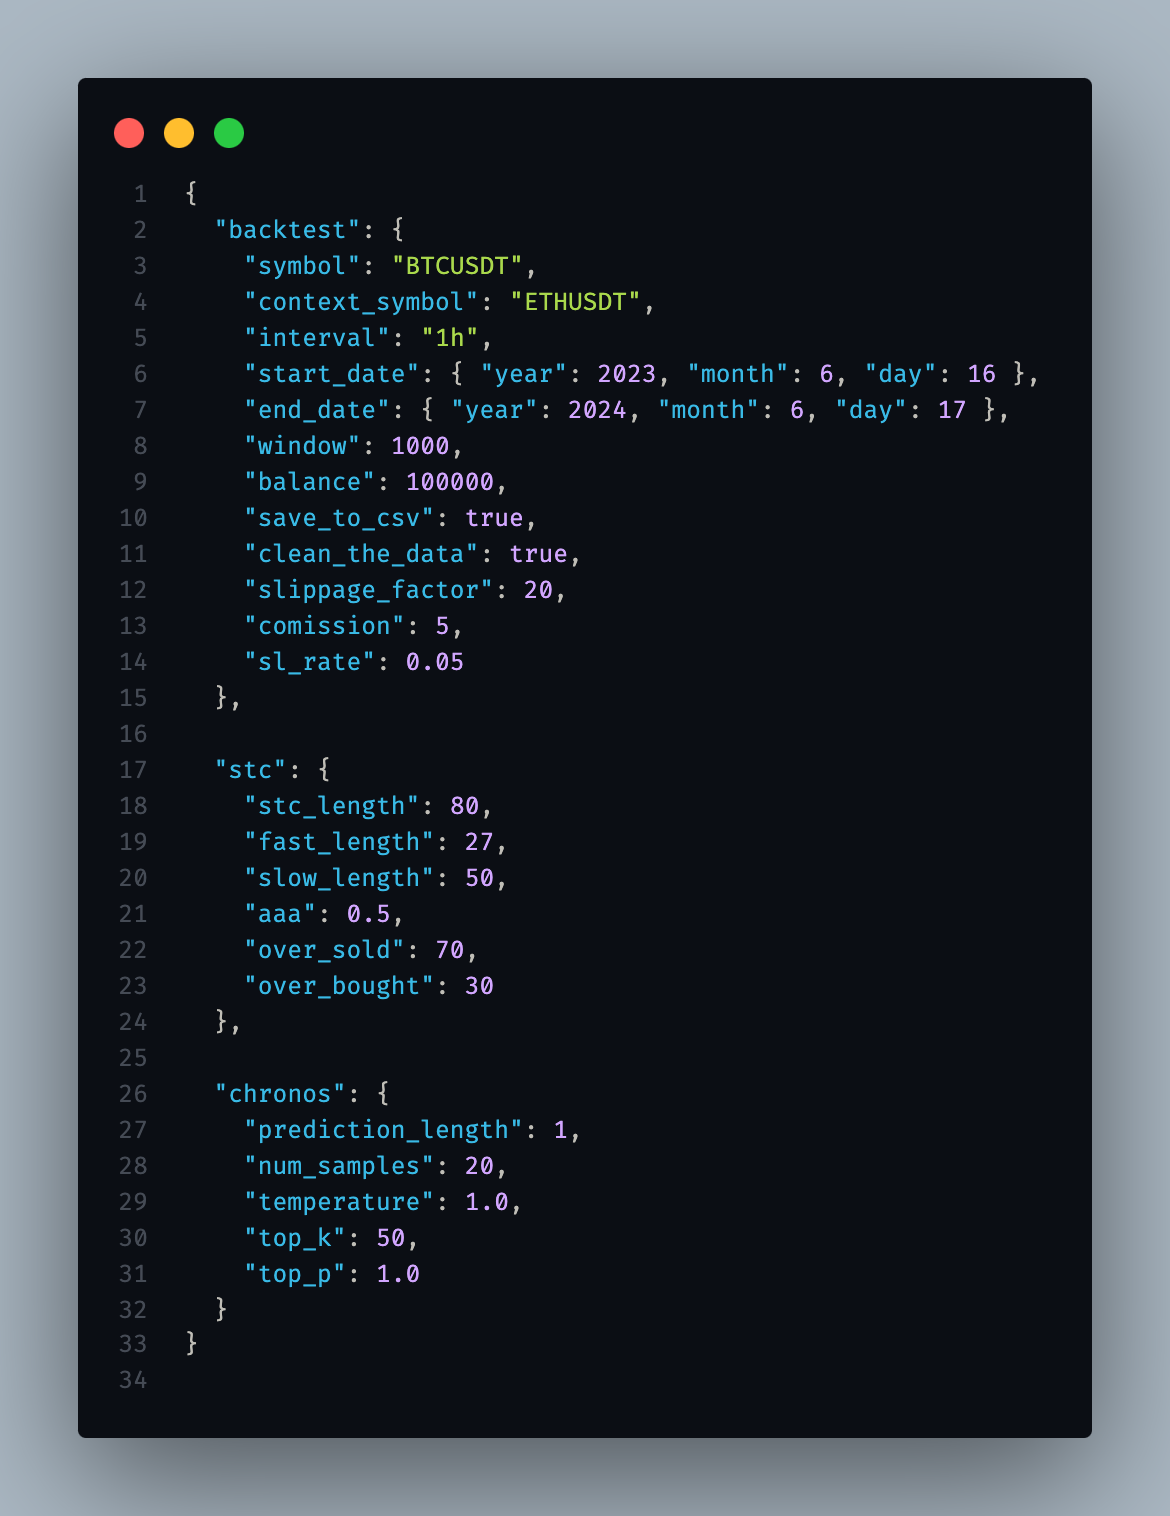
\includegraphics[width=.8\textwidth]{config.png}
    \caption{קובץ \te{config.json}}
\end{figure}

על מנת להריץ את ה\te{Backtesting} יש צורך להריץ את הקובץ \te{main.py}. \\
התוכנית תתחיל בלהוריד את הדאטא בטווח הזמן שנבחר, לאחר מכן היא תבדוק, תנקה ותתקן את דאטא (במידה וזה התבקש על ידי המשתמש בקובץ \te{config.json}). לאחר מכן התוכנית תחשב את הסיגנלים לפי האסטרטגיה והיא תיצור 2 אסטרטגיות בסיסיות (\te{Buy and Hold, Sell and Hold}) כבסיס להשוואה.
לאחר שיש לנו את הסיגנלים, נקרא לפונקציה \te{backtest($\cdot$)}. הפונקציה \te{backtest($\cdot$)} תסמלץ עבורנו את המסחר ולאחר מכן נקרא לפונקציה \te{evaluate\_strategy($\cdot$)} על מנת שהיא תחשב את הרווח ומדדי הביצוע של האסטרטגיה.
\begin{figure}[H]
    \centering
    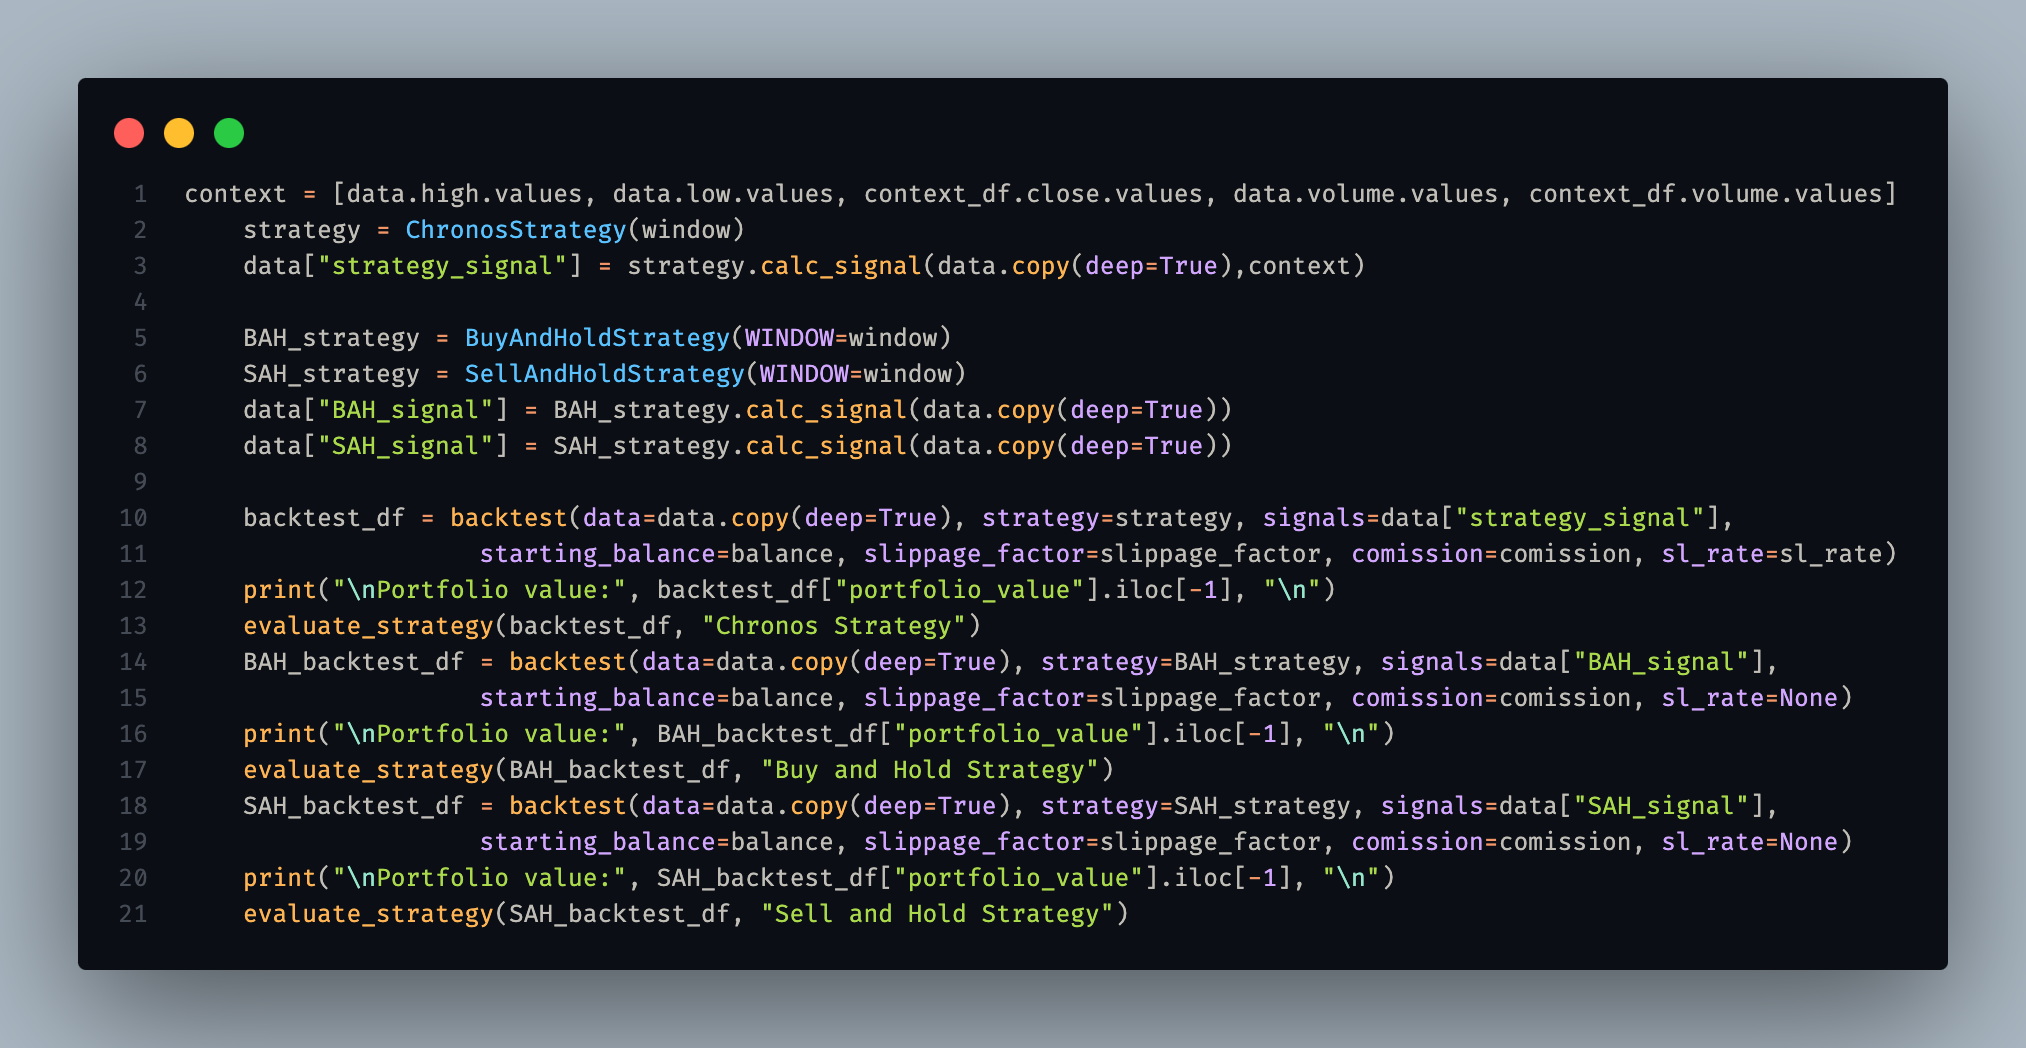
\includegraphics[width=.9\textwidth]{backtesting.png}
    % \caption{פונקציית ה\te{Backtesting}}
\end{figure}
הפונקציה \te{backtest($\cdot$)} תסמלץ מסחר בכך שהיא תעבור שורה שורה על הדאטא. בכל שורה, אם אנחנו בפוזיציה התוכנית תבדוק אם התנאי ל\te{Stop loss / Take profit} התקיים ואם כן היא תסגור את הפוזיציה בהתאם למחירים.
לא משנה אם אנחנו בפוזיציה או לא, היא תבדוק את האיתות לאותה שורה, אם יש איתות קנייה אז היא תבדוק אם אנחנו בפוזיציית \te{short} ואם כן היא תסגור את הפוזיציה, אם לא היא תבדוק אם אנחנו בכלל בפוזיטיציה, אם כן אז לא נעשה דבר, ואם לא תיכנס לפוזיציית \te{long}. אם יש איתות מכירה, אז מתקיים ההפך.
 כשהלולאה מגיעה לשורה האחרונה בדאטא, אם אנחנו בפוזיצייה היא סוגרת אותה.



\begin{figure}[H]
    \centering
    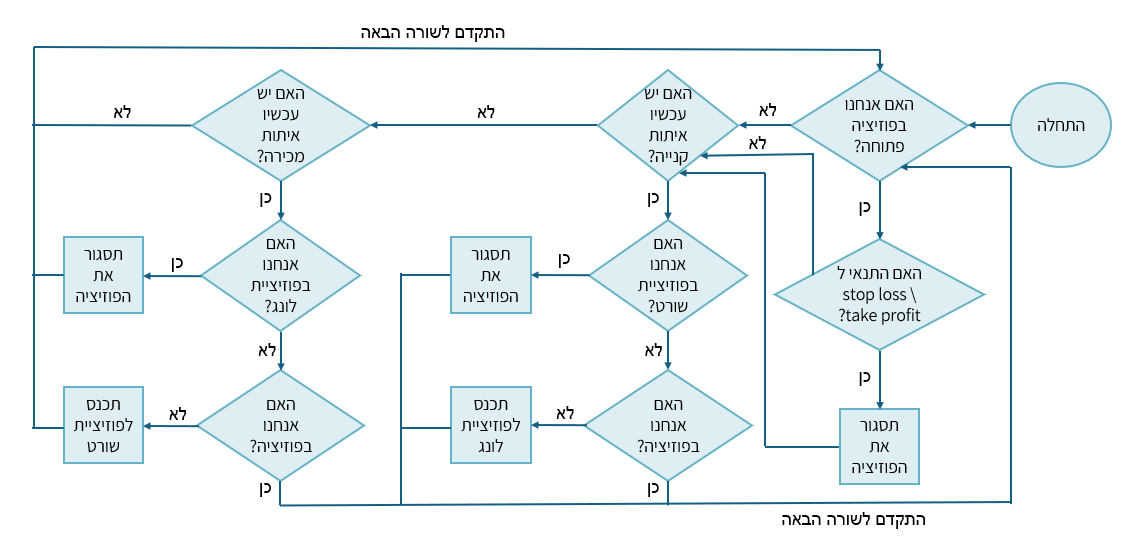
\includegraphics[width=1\textwidth]{flow_chart.png}
    \caption{תרשים זרימה של ה\te{Backtesting}}
\end{figure}
ב \te{backtest} יש גם קריאה לפונקציית \te{calc\_realistic\_price($\cdot$)} מתוך ההבנה שכל פעם שנרצה לעשות עסקה, לא בהכרח נתפוס אותה במחיר שרצינו וגם צריך לקחת בחשבון את עמלות המסחר. כפי שאפשר לראות בקובץ \te{config.json} בחרנו \te{slippage\_factor} של 20, עמלה של 5 דולר לכל מכירה וקנייה. (יש משתנה שסופר את כמות העסקאות ומוריד בסוף תקופת המסחר \te{backtesting} את העמלות מהרווח).
\\ בקובץ \te{config.json} יש אפשרות לבחור אם לשמור את הדאטא והתוצאות לקובץ \te{csv}.
\section{תוצאות}
לאחר ה\te{Backtesting} אנו קוראים לפונקציה \te{evaluate\_strategy($\cdot$)} לכל אחת מהאסטרטגיות, הפונקציה מחשבת את מדדי הביצוע הבאים :
\begin{itemize}
    \item \te{Sharpe Ratio}
    \item \te{Sortino Ratio}
    \item \te{Max Drawdown}
    \item \te{Annualized Return}
    \item \te{Calmar Ratio}
\end{itemize}

\begin{figure}[htbp]
    \centering
    \begin{subfigure}{0.45\textwidth}
        \centering
        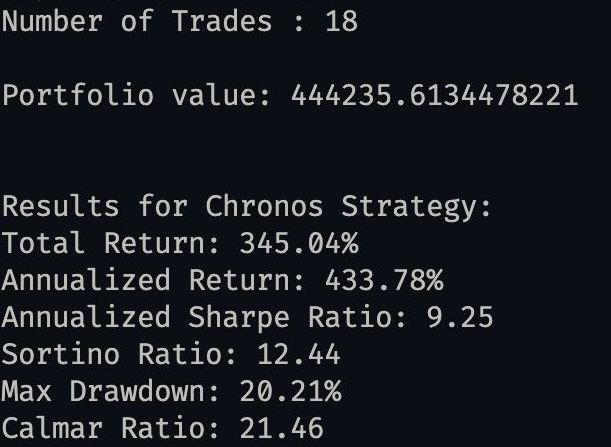
\includegraphics[height=0.8\linewidth]{Results_output.jpeg}
        \caption{ביצועי \te{Chronos}}
        \label{fig:sub1}
    \end{subfigure}
    \hfill
    \begin{subfigure}{0.45\textwidth}
        \centering
        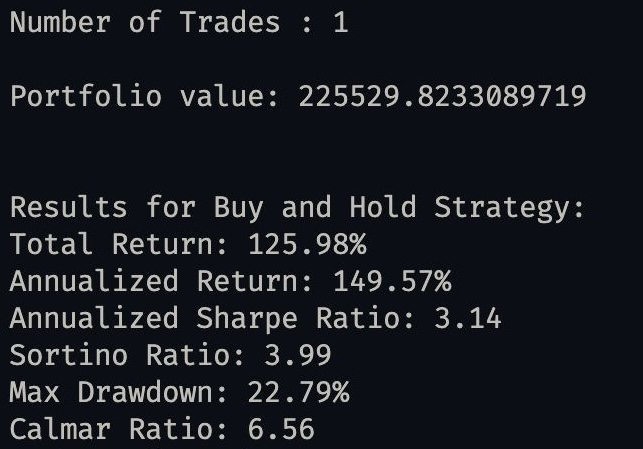
\includegraphics[height=0.8\linewidth]{Results_ouput2.jpeg}
        \caption{ביצועי \te{Buy and Hold}}
        \label{fig:sub2}
    \end{subfigure}
    % \caption{Overall caption for the two figures}
    \label{fig:figures}
\end{figure}
לאחר מכן התוכנית מציגה גרף של השינוי בערך התיק כפונקציה של זמן לכל שלושת האסטרטגיות כדי שנוכל להשוות בין האסטרטגיות. כפי שאפשר לראות בעמוד הבא.

\begin{figure}[H]
    \centering
    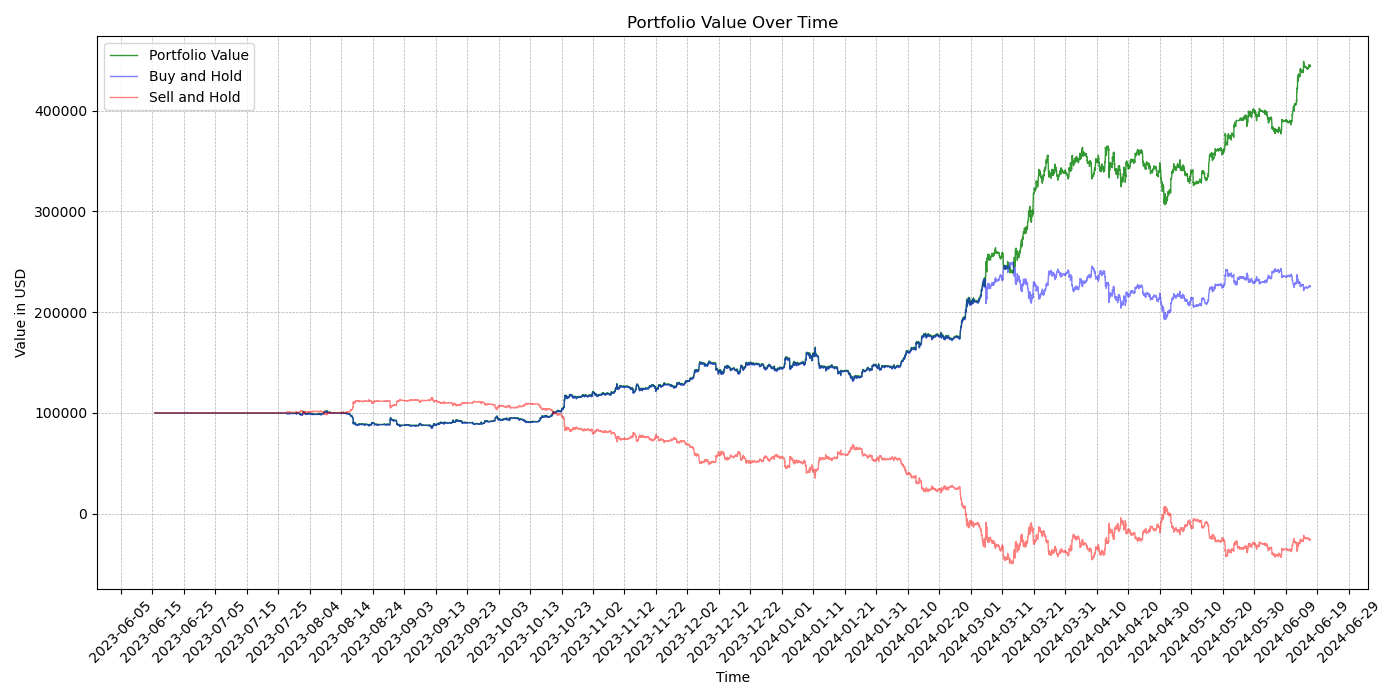
\includegraphics[width=1\textwidth]{backtesting1.png}
    \caption{ערך התיק כפונקציה של זמן}
\end{figure}
\section{ביבליוגרפיה וקישורים}
\begin{itemize}
    \item \href{https://github.com/amazon-science/chronos-forecasting?tab=readme-ov-file}{\te{Chronos - Amazon paper}}
    \item \href{https://www.binance.com/en}{\te{Binance}}
    \item \href{https://github.com/GabrielMagidov/Algotrading}{\te{Our GitHub Repository}}
\end{itemize}
\end{RTL}
\end{document}